
\section{g(x)优点的验证}
\label{sec:benefit}
如Table \ref{tab:accept}所示,$g(x)$的接受率更高,尤其是large step较为显著,这使得不同sds区域之间的亮度比例可以更快收敛。Figure \ref{fig:Grid9PyramidFigMALA}、Figure \ref{fig:Grid100SphereFigH2MC}、Figure \ref{fig:Grid25TeapotFigMALA}分别以\textbf{Grid9Pyramid}、\textbf{Grid100Sphere}、\textbf{Grid25Teapot}为例展示了图片结果。通过error map可以更清晰地看出对于不同区域间亮度比例,$g(x)$收敛得更快,从而验证了上述分析。如Figure \ref{fig:GridPyramidMSE}、Figure \ref{fig:GridSphereMSE}、Figure \ref{fig:GridTeapotMSE}的MSE曲线所示,随着物体数量M的增加,场景中有更多完全不连通的sds区域,$g(x)$的优势更加明显。

\begin{table}[hb]
\centering
\begin{tabular}{|c|c|c|c|c|c|c|c|}
% \hline
% Grid25Pyramid-h2mc & l & l & l & s & s & s\\
\hline
Grid[M]Scene & M & f Large & $g_{1.25}$ Large & $g_{1.5}$ Large & f Small & $g_{1.25}$ Small & $g_{1.5}$ Small \\
\hline
\multirow{4}{*}{Grid[M]Pyramid} & 1 & 0.001351 & 0.002024 & 0.002766 & 0.5064 & 0.5132 & 0.5221\\
\cline{2-8} & 9 & 0.000988 & 0.00148 & 0.00204 & 0.3604 & 0.3631 & 0.3686\\
\cline{2-8} & 25 & 0.001205 & 0.001806 & 0.002492 & 0.290 & 0.2915 & 0.2958\\
\cline{2-8} & 100 & 0.001214 & 0.001809 & 0.002492 & 0.1608 & 0.1618 & 0.1642\\
\hline
\multirow{4}{*}{Grid[M]Sphere} & 1 & 0.0360 & 0.03873 & 0.04123 & 0.3946 & 0.4132 & 0.4339\\
\cline{2-8} & 9 & 0.02481 & 0.0267 & 0.02821 & 0.3589 & 0.3559 & 0.3574\\
\cline{2-8} & 25 & 0.02903 & 0.03135 & 0.03307 & 0.3324 & 0.3271 & 0.3255\\
\cline{2-8} & 100 & 0.02732 & 0.02964 & 0.03144 & 0.3016 & 0.2932 & 0.2878\\
\hline
\multirow{4}{*}{Grid[M]Teapot} & 1 & 0.00583 & 0.006402 & 0.006882 & 0.3478 & 0.3609 & 0.3704\\
\cline{2-8} & 9 & 0.006155 & 0.006661 & 0.007075 & 0.2439 & 0.2509 & 0.2547\\
\cline{2-8} & 25  & 0.007798 & 0.008409 & 0.008967 & 0.2169 & 0.2207 & 0.2224\\
\cline{2-8} & 100 & 0.007922 & 0.008557 & 0.009073 & 0.1880 & 0.1889 & 0.1879\\
\hline
% Grid9Pyramid-mala & 0.000987 & 0.00148 & 0.00204 & 0.2688 & 0.3298 & 0.3780\\
% \hline
% Grid100Sphere-mala & 0.02708 & 0.02941 & 0.03127 & 0.03293 & 0.04783 & 0.06356\\
% \hline
% Grid25Teapot-mala & 0.007857 & 0.008491 & 0.009032 & 0.06045 & 0.08629 & 0.1102\\
% \hline
\end{tabular}
\caption{Grid场景中,H2MC的接受率}
\label{tab:accept}
\end{table}

\clearpage
\begin{figure}
\begin{minipage}{\textwidth}
\centering  
\renewcommand{\arraystretch}{0.35}
\addtolength{\tabcolsep}{-5.0pt}
 \begin{tabular}{ ccccc }
\begin{overpic}[width=\gridMseFigWidth]{\GridMSE{Pyramid}{1}{h2mc}}\end{overpic}
& \begin{overpic}[width=\gridMseFigWidth]{\GridMSE{Pyramid}{4}{h2mc}}\end{overpic}
& \begin{overpic}[width=\gridMseFigWidth]{\GridMSE{Pyramid}{9}{h2mc}}\end{overpic}
& \begin{overpic}[width=\gridMseFigWidth]{\GridMSE{Pyramid}{25}{h2mc}}\end{overpic}
& \begin{overpic}[width=\gridMseFigWidth]{\GridMSE{Pyramid}{100}{h2mc}}\end{overpic}
\\
\begin{overpic}[width=\gridMseFigWidth]{\GridMSE{Pyramid}{1}{mala}}\end{overpic}
& \begin{overpic}[width=\gridMseFigWidth]{\GridMSE{Pyramid}{4}{mala}}\end{overpic}
& \begin{overpic}[width=\gridMseFigWidth]{\GridMSE{Pyramid}{9}{mala}}\end{overpic}
& \begin{overpic}[width=\gridMseFigWidth]{\GridMSE{Pyramid}{25}{mala}}\end{overpic}
& \begin{overpic}[width=\gridMseFigWidth]{\GridMSE{Pyramid}{100}{mala}}\end{overpic}
\\
\end{tabular}
\end{minipage}
\caption{Grid[M]PyramidMSE:Diffuse平面上摆放了M个透明金字塔,从左到右依次是M=1, 4, 9, 25, 100。第一行是h2mc的结果,第二行是mala的结果。图例中C128表示chain数量为128, P0.2表示large step的概率为0.2, roughScale表示$g(x)$对$\alpha$的放大程度,1.0表示$g(x)=f(x)$。从图中可以看到,随着M数量的增加,\textcolor{orange}{$g_{1.25}(x)$}和\textcolor{green}{$g_{1.5}(x)$}会优于\textcolor{blue}{$f(x)$}}
\label{fig:GridPyramidMSE} 
\end{figure}

\begin{figure}
\begin{minipage}{\textwidth}
\centering  
\addtolength{\tabcolsep}{-5.0pt}
 \begin{tabular}{ ccccc }
\begin{overpic}[width=\gridMseFigWidth]{\GridMSE{Sphere}{1}{h2mc}}\end{overpic}
& \begin{overpic}[width=\gridMseFigWidth]{\GridMSE{Sphere}{4}{h2mc}}\end{overpic}
& \begin{overpic}[width=\gridMseFigWidth]{\GridMSE{Sphere}{9}{h2mc}}\end{overpic}
& \begin{overpic}[width=\gridMseFigWidth]{\GridMSE{Sphere}{25}{h2mc}}\end{overpic}
& \begin{overpic}[width=\gridMseFigWidth]{\GridMSE{Sphere}{100}{h2mc}}\end{overpic}
\\
\end{tabular}
\end{minipage}
\caption{Grid[M]SphereMSE:Diffuse平面上摆放了M个透明玻璃球,从左到右依次是M=1, 4, 9, 25, 100。Small Step为H2MC。}
\label{fig:GridSphereMSE} 
\end{figure}

\begin{figure}
\begin{minipage}{\textwidth}
\centering  
\addtolength{\tabcolsep}{-5.0pt}
 \begin{tabular}{ ccccc }
\begin{overpic}[width=\gridMseFigWidth]{\GridMSE{Teapot}{1}{mala}}\end{overpic}
& \begin{overpic}[width=\gridMseFigWidth]{\GridMSE{Teapot}{4}{mala}}\end{overpic}
& \begin{overpic}[width=\gridMseFigWidth]{\GridMSE{Teapot}{9}{mala}}\end{overpic}
& \begin{overpic}[width=\gridMseFigWidth]{\GridMSE{Teapot}{25}{mala}}\end{overpic}
& \begin{overpic}[width=\gridMseFigWidth]{\GridMSE{Teapot}{100}{mala}}\end{overpic}
\\
% \begin{overpic}[width=\gridMseFigWidth]{\GridMSE{Teapot}{1}{h2mc}}\end{overpic}
% & \begin{overpic}[width=\gridMseFigWidth]{\GridMSE{Teapot}{4}{h2mc}}\end{overpic}
% & \begin{overpic}[width=\gridMseFigWidth]{\GridMSE{Teapot}{9}{h2mc}}\end{overpic}
% & \begin{overpic}[width=\gridMseFigWidth]{\GridMSE{Teapot}{25}{h2mc}}\end{overpic}
% & \begin{overpic}[width=\gridMseFigWidth]{\GridMSE{Teapot}{100}{h2mc}}\end{overpic}
% \\
\end{tabular}
\end{minipage}
\caption{Grid[M]TeapotMSE 在Diffuse平面上摆放了M个透明茶壶,从左到右依次是M=1, 4, 9, 25, 100。Small Step为MALA。}
\label{fig:GridTeapotMSE} 
\end{figure}
\begin{figure}
\begin{minipage}{\textwidth}
\centering  
\addtolength{\tabcolsep}{-5.0pt}
\begin{tabular}{c}
\begin{overpic}[width=\ResultFigWidth]{\GridFig{Pyramid}{9}{mala}}\end{overpic} \\
\begin{overpic}[width=\ResultFigWidth]{\GridErrFig{Pyramid}{9}{mala}}
    \put(14.3, 0){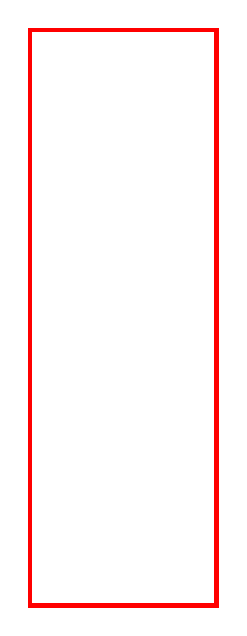
\begin{tikzpicture}[x=1pt,y=1pt]
        \draw[red,ultra thick] (0,0) rectangle (67.5,208);
    \end{tikzpicture}}
    \put(28.7, 0){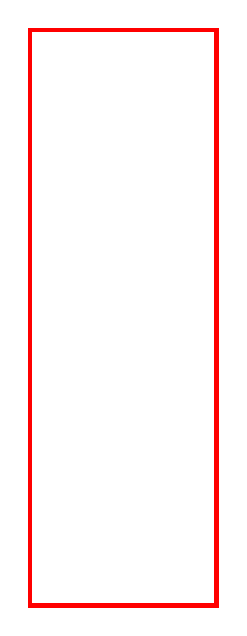
\begin{tikzpicture}[x=1pt,y=1pt]
        \draw[red,ultra thick] (0,0) rectangle (67.5,208);
    \end{tikzpicture}}
    \put(43, 0){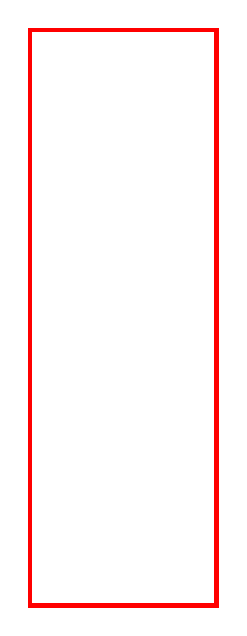
\begin{tikzpicture}[x=1pt,y=1pt]
        \draw[red,ultra thick] (0,0) rectangle (67.5,208);
    \end{tikzpicture}}
\end{overpic} \\
\end{tabular}
\end{minipage}
\caption{Grid9Pyramid-MALA: 第一行为$f(x)$的结果,第二行为$g_{1.25}(x)$,第三行为$g_{1.5}(x)$。后三行是对应的error map。通过error map的第二三四列都可以看出,$f(x)$的error map的区域间相对亮度误差更大。}
\label{fig:Grid9PyramidFigMALA}
\end{figure}

\begin{figure}
\begin{minipage}{\textwidth}
\centering  
\addtolength{\tabcolsep}{-5.0pt}
\begin{tabular}{c}
\begin{overpic}[width=\ResultFigWidth]{\GridFig{Sphere}{100}{h2mc}}\end{overpic} \\
\begin{overpic}[width=\ResultFigWidth]{\GridErrFig{Sphere}{100}{h2mc}}
    \put(7.4, 34.2){
\begin{tikzpicture}[x=1pt,y=1pt]
        \draw[red, thick] (0,0) rectangle (10,10);
    \end{tikzpicture}}
    \put(21.8, 34.2){
\begin{tikzpicture}[x=1pt,y=1pt]
        \draw[red, thick] (0,0) rectangle (10,10);
    \end{tikzpicture}}
    \put(36.2, 34.2){
\begin{tikzpicture}[x=1pt,y=1pt]
        \draw[red, thick] (0,0) rectangle (10,10);
    \end{tikzpicture}}
    \put(38.7, 31.7){
\begin{tikzpicture}[x=1pt,y=1pt]
        \draw[red, thick] (0,0) rectangle (10,10);
    \end{tikzpicture}}
    \put(50.6, 34.2){
\begin{tikzpicture}[x=1pt,y=1pt]
        \draw[red, thick] (0,0) rectangle (10,10);
    \end{tikzpicture}}
    \put(53.1, 31.7){
\begin{tikzpicture}[x=1pt,y=1pt]
        \draw[red, thick] (0,0) rectangle (10,10);
    \end{tikzpicture}}
    \put(65, 34.2){
\begin{tikzpicture}[x=1pt,y=1pt]
        \draw[red, thick] (0,0) rectangle (10,10);
    \end{tikzpicture}}
    \put(11.3, 16.2){
\begin{tikzpicture}[x=1pt,y=1pt]
        \draw[red, thick] (0,0) rectangle (10,10);
    \end{tikzpicture}}
    \put(25.7, 16.2){
\begin{tikzpicture}[x=1pt,y=1pt]
        \draw[red, thick] (0,0) rectangle (10,10);
    \end{tikzpicture}}
\end{overpic} \\
\end{tabular}
\end{minipage}
\caption{Grid100Sphere-H2MC: 通过error map可以看出,$g_{1.25}(x)$和$g{1.5}(x)$相较于$f(x)$,各个区域亮度分配更均匀。}
\label{fig:Grid100SphereFigH2MC} 
\end{figure}

\begin{figure}
\begin{minipage}{\textwidth}
\centering  
\addtolength{\tabcolsep}{-5.0pt}
\begin{tabular}{c}
\begin{overpic}[width=\ResultFigWidth]{\GridFig{Teapot}{25}{mala}}\end{overpic} \\
\begin{overpic}[width=\ResultFigWidth]{\GridErrFig{Teapot}{25}{mala}}\end{overpic} \\
\end{tabular}
\end{minipage}
\caption{Grid25Teapot-MALA 这一场景中茶壶来自veachdoor中的mesh,从MSE来看,$g(x)$仍然优于$f(x)$的结果。}
\label{fig:Grid25TeapotFigMALA}
\end{figure}

\clearpage



